% !TEX root = CSL 2021.tex


In the previous section we showed how to associate each simple type $A$ with a  partial metric $d_{A}$ over the closed terms of type $A$. 
We  now illustrate through a few basic examples how the higher-order and metric features of this semantics can be used to formalize contextual reasoning about program differences.
To make our examples more realistic, we will consider some natural extensions of $\STLC$.

It is not difficult to see that all constructions from Section 3 scale well to any extension of $\STLC$ obtained by adding new base types. For example, we can add to our language a type $\mathsf{Nat}$ for natural numbers, indicating for each $n\in \mathbb N$, the corresponding normal forms of $\mathsf{Nat}$ as $\mathtt n$. A natural choice is to let   
$\intervals{\mathsf{Nat}}=\{ \{ t \mid \exists n\in a \ t\leadsto \mathtt n\}\mid a \text{ finite subset of }\mathbb N \text{ or }a=\mathbb N\}$, $\distances{\mathsf{Nat}}=\mathbb R^{+\infty}$ and $d_{\mathsf{Nat}}(t,u)=| n-m|$, where $t\to^{*}_{\beta}\mathtt n$ and $u\to^{*}_{\beta}\mathtt m$. 

Moreover, the constructions scale well also to extensions of $\STLC$ obtained by adding new program constructors, as soon as these do not compromise the normal form property (since the fact that closed programs of type $\mathsf{Real}$ have a normal form plays an important role in defining the set $\intervals{\mathsf{Real}}$).  
For instance, if we suppose that all programs of type $\mathsf{Real}\to\mathsf{Real}$ in $\STLC$ are either 
differentiable or integrable (see Remark \ref{rem:continuous}), we can consider extension of $\STLC$ with  differential or integral operators, as in $\mathsf{Real\ PCF}$ \cite{Di-Gianantonio:2013aa, Edalat:2000aa}.






\begin{example}[Taylor approximation]

We make the assumption that all programs of type $\mathsf{Real}\to\mathsf{Real}$ in $\STLC$ are differentiable and that for all $n$, we can define a term $\mathtt T^{n}: ((\mathsf{Real}\to \mathsf{Real})\times \mathsf{Real})\to \mathsf{Real}\to \mathsf{Real}$ such that $\mathtt T^{n}\langle f, r\rangle$ computes the $n$-th truncated Taylor expansion of $f$ at $r$. 
Then, given a term $t: \mathsf{Real}\to \mathsf{Real}$, the distance 
$d_{\mathsf{Real}\to\mathsf{Real}}(t, \mathtt T^{n}\langle t,\mathtt 0 \rangle)$ is the map associating an interval $a$ with the diameter of $t(a)\vee (\mathtt T^{n}\langle t,\mathtt 0 \rangle)(a)$. 
The difference between this value and the self-distance of $t$ will approximate 0 when $a$ is a small interval of $0$, and will tend to diverge when $a$ contains points which are far enough from 0. 

%between $t$ and its Taylor expansion within a context  $\mathsf C[\ ]= [\ ] r$ which applies them to some value $r$, can be computed as a function of the interval $[0,r]$.   
For example, if $t$ is the function $t=\lambda x.\sin(x)$, and $a$ is an interval of $0$, then using standard analytic reasoning we can compute a bound
$d_{\mathsf{Real}\to \mathsf{Real}}(t, \mathtt T^{n}\langle t,\mathtt 0 \rangle)(a  )\leq \frac{\diam_{\mathsf{Real}}(a)^{n+1}}{(n+1)!} $, which tends to $0$ as the diameter of $a$ tends to $0$.

Observe that if, instead, we used the $\sup$-distance $d_{\sup}(t,u)= \sup\{d_{\mathsf{Real}}(tr, ur)\mid r\in \Lambda_{\mathsf{Real}}\}$, then we could not reason as above since  
$d_{\sup}(\lambda x.\sin(x), \mathtt T^{n} \langle \lambda x.\sin(x),0\rangle)=\infty$ (as illustrated in Fig. \ref{fig:sintaylor}).  

We can use the higher-order structure of our semantics to push abstraction a bit further. For instance, we can define an approximate program 
$c[y_{1},y_{2}]=\left( \partial (\mathtt T^{n})\langle y_{1}, \tointerval{0}\rangle\right) y_{2}: \intervals{\mathsf{Real}\to \mathsf{Real}}\to \intervals{\mathsf{Real}}\to \intervals{\mathsf{Real}}$ which describes the sensitivity of the $n$-th Taylor expansions in 0. Given two programs $t$ and $u$ and a small interval $a$ of $0$, the real number $c[\partial(t)\vee \partial(u),a]$ measures how much the error of replacing the Taylor expansions of $t$ with the Taylor expansion of $u$ in $0$ diverges from the error produced by simply replacing  $t$ and $u$, when these are applied close to $0$. 
  
\end{example}

\begin{figure}
\begin{subfigure}{0.58\textwidth}
\parbox[h][3cm][c]{\textwidth}{
\adjustbox{center, scale=0.9}{$
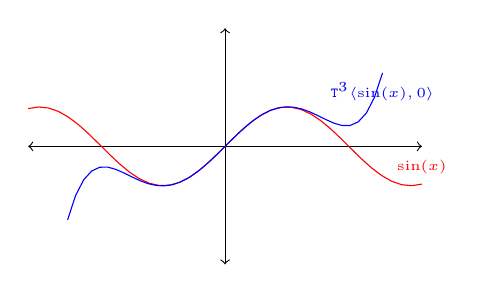
\begin{tikzpicture}[domain=-5:5, scale=0.5]
%\draw[very thin,color=gray] (-0.1,-1.1) grid (3.9,3.9);
\draw[<->]   (-5,0) -- (5,0);
\draw[<->] (0,-3) -- (0,3); % node[above] {$f(x)$};

   % \node at (0,0)[circle,fill,inner sep=1pt]{};
%
\draw[color=red, domain=-5:5, samples=40] plot (\x, {sin(\x r) } ) node[above] {\tiny$\sin(x)$};

\draw[color=blue, domain=-4:4, samples=40] plot (\x,{\x -((\x)^3)/6 + ((\x)^5/120  } ) node[below] {\tiny$\mathtt T^{3}\langle\sin(x),0\rangle$};


\end{tikzpicture}$}
}
\caption{\small The $\sup$-distance between $\sin(x)$ and its Taylor expansion $\mathtt T^{3}\langle\sin(x),0\rangle$ diverges.}
\label{fig:sintaylor}
\end{subfigure} \ \ \ 
\begin{subfigure}{0.4\textwidth}
\parbox[h][3cm][c]{\textwidth}{
\adjustbox{scale=0.45}{$\ \qquad\qquad
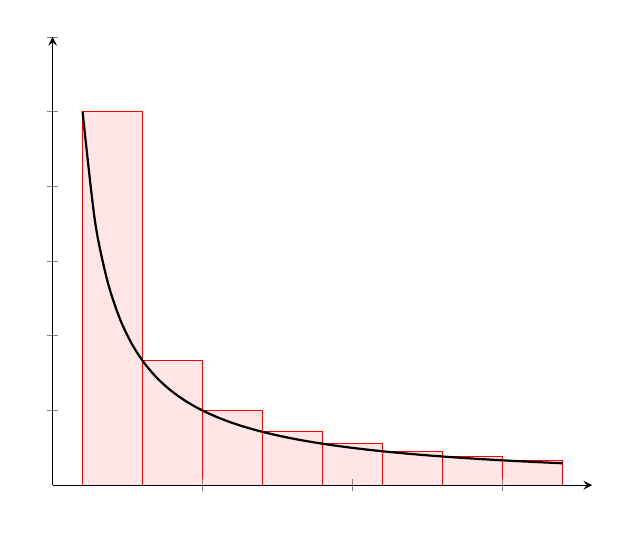
\begin{tikzpicture}
\begin{axis}[
    xticklabels={ , , },yticklabels={ , , },
    xmax=18,ymax=1.2,ymin=0,xmin=0,
    enlargelimits=true,
    axis lines=middle,
    clip=false,
    domain=0:17,
    axis on top
    ]

\addplot [draw=red, fill=red!10, ybar interval, samples=9, domain=1:17]
    {x^-1}\closedcycle;
%\addplot [draw=green, fill=green!10, ybar interval, samples=9, domain=17:1]
  %  {x^-1}\closedcycle;

\addplot[smooth, thick,domain=1:17,samples=40]{x^-1};

\end{axis}
\end{tikzpicture}
$}
%
%\begin{tikzpicture}[scale=0.7,
%    declare function={
%        f(\x)=2+sin(deg(\x-2))+sin(deg(3*\x))/2+sin(deg(5*\x))/8 + sin(deg(7*\x))/28;
%    }
%]
%\begin{axis}[
%    axis lines = middle,
%    %xtick ={1,1.5,2,2.5,3,3.5,4},
%    ytick ={0},
%    %xticklabels = {$a=x_0$,$x_1$,$x_2$,$x_3$, $\ldots$, $x_{n-1}$,$x_n=b$},
%    ymin = -0.2,
%    ymax = 3.7,
%    xmin = -0.2,
%    xmax = 5.2,
%    x=3cm,y=2cm,
%    axis line style = thick,
%    %xlabel={$x$},
%    %ylabel={$y$},
%    %extra x ticks={1.3,1.85,2.2,2.7,3.2,3.75},
%extra x tick labels={$\xi_1$, $\xi_2$, $\xi_3$, $\xi_4$, $\xi_{n-1}$, $\xi_n$},
%]
%
%\addplot [
%    domain=1:4,
%    samples=300,
%    line width=1pt,
%    fill=red, draw=none,
%    fill opacity=0.1
%] {f(x)} \closedcycle;
%
%\addplot [
%    domain=0:5,
%    samples=300,
%    line width = 1pt, red] {f(x)};
%
%\addplot [
%    ycomb, thick, red,
%    no markers,
%    samples at={1,1.5,...,4}
%] {f(x)};
%
%\addplot [
%    ycomb, thick, blue,
%    no markers,
%    samples at={1.3,1.85,2.2,2.6,3.2,3.65}
%] {f(x)};
%
%\addplot[ybar, bar width=30pt, domain=1:4,
%samples at={1.3,1.85,2.2,2.6,3.2,3.65}, fill=blue!50!cyan,fill opacity=0.3, draw=cyan]
%  {f(x)};
%
%
%\end{axis}
%\end{tikzpicture}$}
}
\caption{\small Definite integral $vs$ Riemann sums. \\ \   }
\label{fig:riemann}
\end{subfigure}
\caption{Computing bounds on distances: examples.}
\end{figure}


\begin{example}[Integral approximation]
We now assume that all functions in $\mathcal F_{n}$ are integrable and that we have (see \cite{Edalat:2000aa}) at our disposal a program $\lambda fx.\mathsf I_{[0,x]}(f): (\mathsf{Real}\to \mathsf{Real})\to \mathsf{Real}\to \mathsf{Real}$ such that $\mathsf I_{[0,r]}(t)$ computes (a precise enough approximation of) the definite integral $\int_{0}^{|r|}tx \ dx$.
In many contexts we might prefer to replace the expensive computation of $\mathsf I_{[0,r]}(t)$ by the (more economical but less precise) computation of a finite Riemann sum $\mathsf R^{n}_{[0,r]}(t)=  \sum_{i=1}^{n}(tx_{i})\cdot |r|/n$, where 
 $x_{i}=  i\cdot |r|/n$ (see Fig. \ref{fig:riemann}).  

%
%
%When the second derivative $D^{(2)}t$ of a program $t$ exists (and can be computed efficiently) and moreover is bounded by $M$ on $[0,r]$, the error of replacing the true integral  $\int_{0}^{r}tx dx$ (that we suppose $\mathtt I_{[0,r]}$ is close enough to) by its approximation through a finite Riemann sum, can be bounded
% as $d_{\mathsf{Real}}(\mathsf I_{[0,r]}t, \mathsf R^{n}_{[0,r]}t)\leq  M\cdot |r|^{3}/24n^{2}$.


Suppose now that, in order to approximate the integral of some computationally expensive program $t$ on $[0,r]$, we replace $t$ by some more efficient program $u$ which, over $[0,r]$, is very close to $t$. Let $\epsilon_{t}(r)$ indicate the distance between the true integral of $t$ over $[0,r]$ and $\mathsf{R}^{n}_{[0,r]}(t)$,
 and moreover let 
$\eta_{t,u}(r)$ be the diameter of $\partial(t)([0,r])\vee\partial(u)([0,r])$.

Using the metric structure of $\mathsf{Real}$ we can then bound the error we incur in by replacing the true integral \emph{of $t$} with the Riemann sum \emph{of $u$}. 
In fact, by standard calculation we can compute the bound
$d_{\mathsf{Real}} ( \mathsf{R}^{n}_{[0,r]}(t), \mathsf R^{n}_{[0,r]}(u))\leq 
d_{\mathsf{Real}\to\mathsf{Real}}(t, u)([0,r]) \cdot n \cdot |r|=\eta_{t,u}(r)\cdot n \cdot |r|$.
Then, using the triangular inequality of the standard metric on $\mathsf{Real}$ we deduce
\begin{align*}
 d_{\mathsf{Real}} ( \mathsf{I}_{[0,r]}(t), \mathsf R^{n}_{[0,r]}(u)) \leq
d_{\mathsf{Real}} ( \mathsf{I}_{[0,r]}(t), \mathsf R^{n}_{[0,r]}(t))  & +
d_{\mathsf{Real}} ( \mathsf{R}_{[0,r]}(t),\mathsf R^{n}_{[0,r]}(u)) \\
& \leq \epsilon_{t}(r)
+ 
\eta_{t,u}(r)\cdot 
 n\cdot |r|
 \end{align*}
 Using the partial metric on $\mathsf{Real}\to \mathsf{Real}$, we can also derive a bound expressing how much the error above is \emph{sensitive to changes of $r$}. 
First, using standard analytic techniques (under suitable assumptions for $t$ and its derivatives) one can find a program $v:\mathsf{Real}\to\mathsf{Real}$ such that $vr \to^{*}_{\beta}\epsilon_{t}(r)$. 
Then, using the triangular inequality of the partial metric on $\mathsf{Real}\to \mathsf{Real}$ we deduce, for all interval $a$, the following bound:
\begin{align*}
& d_{\mathsf{Real}\to\mathsf{Real}} (\lambda x. \mathsf{I}_{[0,x]}(t),\lambda x. \mathsf R^{n}_{[0,x]}(u))(a) \\
 &\leq \
d_{\mathsf{Real}\to\mathsf{Real}} ( \lambda x.\mathsf{I}_{[0,x]}(t), \lambda x.\mathsf R^{n}_{[0,x]}(t))(a) +
d_{\mathsf{Real}\to\mathsf{Real}} ( \lambda x.\mathsf{R}_{[0,x]}(t), \lambda x.\mathsf R^{n}_{[0,x]}(u))(a) \\
 & \qquad\qquad\qquad\qquad\qquad\qquad\qquad\qquad\qquad\qquad
- d_{\mathsf{Real}\to\mathsf{Real}} ( \lambda x.\mathsf{R}_{[0,x]}(t), \allowbreak \lambda x. \mathsf R^{n}_{0,x]}(t))(a) \\
 & \leq \ 
 %\Big(
d_{\mathsf{Real}\to \mathsf{Real}}(v,v)(a)
 %\diam_{\mathsf{Real}}(\partial(\lambda x.\epsilon_{t}(x))(y))
 +
 \big( d_{\mathsf{Real}\to\mathsf{Real}}(t,u)(a)- d_{\mathsf{Real}\to\mathsf{Real}}(t,t)(a)\big)\cdot n\cdot \diam_{\mathsf{Real}}(a)
 %\Big)
%  \bigg ( 
%\diam_{\mathsf{Real}}\Big ( \big (\partial(\mathsf I_{[0,\_]})\partial(t)y\big ) \vee \big (\partial(\mathsf I_{[0,\_]})\partial(u)y\big)\Big ) \\
% & \qquad\qquad\qquad\qquad\qquad\qquad
%+
%\big(\diam_{\mathsf{Real}} (\partial(t)(y)\vee \partial(u)(y))- \diam_{\mathsf{Real}} (\partial(t)(y))\big)\cdot n \cdot \diam_{\mathsf{Real}}(y)\bigg)
%% 
% \ ??(\varepsilon_{t})
%+ 
%(\partial(\eta_{t,u})(x)-\partial(\eta_{t,t})(x))\cdot 
% n\cdot \diam_{\mathsf{Real}}(x)
\end{align*}
\end{example}



%using the triangular inequality of partial metrics, we can deduce a bound for the distance 
%$ d_{\mathsf{Real}\to\mathsf{Real}} (\lambda x. \mathsf{I}_{[0,x]}t,\lambda x. \mathsf R^{n}_{[0,x]}u)\in \intervals{Real}\to \distances{Real}$ by 
%$d_{\mathsf{Real}\to\mathsf{Real}} (\lambda x. \mathsf{I}_{[0,x]}t,\lambda x. \mathsf R^{n}_{[0,x]}u)
%\leq
%d_{\mathsf{Real}\to\mathsf{Real}} ( \lambda x.\mathsf{I}_{[0,x]}t, \lambda x.\mathsf R^{n}_{[0,x]}t) +
%d_{\mathsf{Real}\to\mathsf{Real}} ( \lambda x.\mathsf{R}_{0,x]}t, \lambda x.\mathsf R^{n}_{0,x]}u) -
%d_{\mathsf{Real}\to\mathsf{Real}} ( \lambda x.\mathsf{R}_{0,x]}t,\lambda x. \mathsf R^{n}_{0,x]}t)
%\leq 
%\epsilon_{t,a}
%+ 
%(\delta_{t,u,a}-\delta_{t,t,a})\cdot 
% n\cdot \diam_{\mathsf{Real}}(a)
%$.

%
%+\lambda x. \mathsf{R}_{x}u, \mathsf R^{n}_{x}t)
%\leq 
%
% d_{\mathsf{Real}} ( \mathsf{I}_{r,s}f, \mathsf R^{n}_{r,s}f)+
%  d_{\mathsf{Real}} ( \mathsf{R}^{n}_{r,s}f, \mathsf R^{n}_{r,s}f)\leq 
% H(f'',n)+
%d_{\mathsf{Real}\to\mathsf{Real}}(f, g)([r,s]) \cdot n (\Delta x)^{n}
%$.
%
%
%
% some program $t$ for which we know that the Riemann sum approximates the real integral with a small error $\epsilon_{t}$, and 
%
% program $u$ which is close to $t$ between $r$ and $s$, but for which we cannot compute directly a bound for $\epsilon_{u}=d_{\mathsf{Real}}(\mathsf I_{r,s}u, \mathsf R^{n}_{r,s}u)$ (for example, because second derivatives do not exist or cannot be computed efficiently). Then we can use higher-order reasoning, along with the partial metric structures to compute a bound for $\delta_{u}$.
%
%Then, 
%
%
%
%
%What then if one starts from \emph{different} programs $t,u:\mathsf{Real}\to \mathsf{Real}$ and wants to
%bound the distance
%, the distance between the real integral of $\mathtt I_{r,s}f$ of $f$ and the approximate integral $\mathtt R^{n}_{r,s}g$ of $g$, supposing $f$ and $g$ are close each other on the interval $[r,s]$. 
% In fact, by standard calculation we can compute the bound
%$d_{\mathsf{Real}} ( \mathsf{R}^{n}_{r,s}f, \mathsf R^{n}_{r,s}g)\leq 
%d_{\mathsf{Real}\to\mathsf{Real}}(f, g)([r,s]) \cdot n (\Delta x)^{n}
%$, which is small for small values of $|r-s|$. Then,
% using the triangular inequality we obtain an explicit bound
%$d_{\mathsf{Real}} ( \mathsf{I}_{r,s}f, \mathsf R^{n}_{r,s}g)\leq
% d_{\mathsf{Real}} ( \mathsf{I}_{r,s}f, \mathsf R^{n}_{r,s}f)+
%  d_{\mathsf{Real}} ( \mathsf{R}^{n}_{r,s}f, \mathsf R^{n}_{r,s}f)\leq 
% H(f'',n)+
%d_{\mathsf{Real}\to\mathsf{Real}}(f, g)([r,s]) \cdot n (\Delta x)^{n}
%$.

%As in the previous example, we could not use the distance between $f$ and $g$ in a relevant way if this were the $\sup$-distance, since, although close on $[r,s]$, $f$ and $g$ might get arbitrarily far from each other over all reals. 



\begin{example}[Loop perforation]
By adapting an example from \cite{chaudhuri}, we discuss a simplified example of the transformation that replaces a program $t$ which performs $n$-iterations by a program which only performs the iterations $0,k,2k,3k,\dots$, each repeated $k$ times. We work in the extension of $\STLC$ with a type $\mathsf{Nat}$.




%Let $\mathsf{Nat}$ be a suitable type representing natural numbers in $\STLC$ and s
Suppose  $t: (A\times A\to A) \to \mathsf{Nat}\to (A\to A)\to A$, for $n\geq 1$, is a term such that $th\mathtt n f$ 
computes the $n$-times iteration of $h$ as follows: $th \mathtt 0f= h\langle f\mathtt 0, f\mathtt 0\rangle$ and $th(\mathtt{n+1})f=h\langle th\mathtt n f, f\mathtt{n+1}\rangle$. 
Let $\mathsf{Perf}^{k}(t)$, the $k$-th perforation of $t$, be the program   
$(\mathsf{Perf}^{k}(t))h\mathtt nf= t(\lambda x. (h^{(k)}x)) \mathtt{\lfloor n\rfloor_{k}} (\lambda x. f(x* \mathtt k)$, where $\lfloor n\rfloor_{k}$ indicates the least $m\leq n$ such that $m$ is divisible by $k$, and $x*\mathtt k$ is the multiplication of $x$ by $k$. 





To compute the distance 
$d_{A}(v_{n},w_{n}    )$ between  $v_{n}=th\mathtt n f $ and its perforation $w_{n}=\mathsf{Perf}^{k}(t)h\mathtt nf$  we can reason as follows: 
\begin{itemize}

\item[i.] $v_{n}$ performs $n$-iterations while $w_{n}$ performs $k\lfloor n\rfloor_{k}  \leq n$ iterations, and we can compute  
$d_{A}(v_{n}, v_{(k \lfloor n\rfloor_{k})})$ as the diameter of 
$\partial(t)\partial(h)([ k \lfloor n\rfloor_{k}, n]_{\mathsf{Nat}}) \partial(f)$.




\item[ii.] If $n$ is divisible by $k$, then for $i\leq n$, at the $i$-th iteration of $v_{n}$ the function $f$ is applied  to $\mathtt i$, while at the $i$-th iteration of $w_{n}$, $f$ is applied to $\lfloor i\rfloor_{k}$. Now, the error of replacing  $f\mathtt i$ by $ f\lfloor \mathtt j\rfloor_{k}$, with $\mathtt i,\mathtt j$ in some $a\in \intervals{\mathsf{Nat}}$, is accounted for by the approximate program $c[y]= \partial(f)(y-k  )$, where $y-k= y \vee \{u-\mathtt k\mid u \in y\}$.
We deduce then that 
$d_{A}(v_{n}, w_{n})$ is bounded by the diameter of $\partial(t)\partial(f)\tointerval{\mathtt n} (\lambda y.c[y])$.

\item[iii.] From the fact that $w_{n}=w_{(k\cdot \lfloor n\rfloor_{k})}$ and the triangular inequality of the partial metric $d_{A}$ we deduce  
$d_{A}(v_{n}, w_{n})=
d_{A}(v_{n},w_{(k\cdot \lfloor n\rfloor_{k})}) \leq
d_{A}(v_{n}, v_{(k\cdot \lfloor n\rfloor_{k})})+
d_{A}(v_{(k\cdot \lfloor n\rfloor_{k})}, w_{(k\cdot \lfloor n\rfloor_{k})})-
d_{A}(v_{(k\cdot \lfloor n\rfloor_{k})},v_{(k\cdot \lfloor n\rfloor_{k})} )$


\end{itemize}

From facts i.-iii. we immediately deduce an explicit bound for $d_{A}(v_{n},w_{n}    )$ as a function of $\partial(t), \partial(f)$ and $n$. 

\end{example}

%
% $\partial(t)   \partial(h) \tointerval{\mathtt n} (\lambda x.\partial (f)(x-k))$.

%{
%
%given by $\mathsf{Perf}^{k}(t^{0})f= t^{0}f$ and $\mathsf{Perf}^{k}(t^{n+1})f=
%h( \mathsf{Perf}^{k}(t^{n})f, f \mathtt{\lfloor n+1/k\rfloor})$ if ${\lfloor n+1/k\rfloor}> {\lfloor n/k\rfloor}$, and $\mathsf{Perf}^{k}(t^{n+1})f=\mathsf{Perf}^{k}(t^{n})f$ otherwise.
%
%
%While $d_{A}(t^{1}f, \mathsf{Perf}^{k}(t^{1}f))$ is the self-distance of $t^{1}f\oeq_{\mathsf{A}}f\mathtt 0$ (which is equal to $0$ if, say, $A=\mathsf{Real}$), f

%
%
%As soon as we have a bound  $\rho: a,\mathtt n \mapsto \partial(h)(a,\tointerval{\mathtt n}) \vee a$
% for the smallest interval containing a value $t:A$ and its image $h(t,\mathtt n)$, we  can  compute explicit bounds for  the distance $d_{A}(t^{n}f,\mathsf{Perf}^{k}(t^{n})f)$. In fact, by letting $D_{A}(u,v): a\mapsto \tointerval u\vee \tointerval v$ and recalling that $d_{A}(u,v)=\diam_{A}(D_{A}(u,v))$, we can use the following lemma. 
%\begin{lemma}
%$D_{A}(t^{n+1}f, \mathsf{Perf}^{k}(t^{n+1})f)\leq H(n, \rho, \partial(h), \partial(f), D_{A}(t^{n}f,  \mathsf{Perf}^{k}(t^{n})f))$, where 
%%$\phi=d_{\mathsf{Real}\to \mathsf{Real}}(h,h)$, $\psi= d_{\mathsf{Real}\to \mathsf{Real}}(f,f) $ and , where $H(\phi,\psi,\Phi) $ is
%$H(n,\rho,\phi,\psi, \chi)=
%  \rho^{n}(\tointerval{f\mathtt 0})
%  +
%  \chi
%  +
% \psi( \chi, \psi (\mathtt{n+1},\mathtt{ \lfloor n+1/k\rfloor} ))
%$ and $\rho^{n}(a)$ is defined by $\rho^{0}(a)=a$ and $\rho^{n+1}(a)=\rho(\rho^{n}(a),\mathtt n)$.  
%%
%%In fact, since $t^{n+1}f= h \langle t^{n}f,  f\mathsf{n+1}  \rangle$ and 
%%$\mathsf{Perf}^{k}(t^{n+1})f$ is either equal to $\mathsf{Perf}^{k}(t^{n})f$, if $\lfloor n+1/k\rfloor=\lfloor n/k\rfloor$, or 
%%to $ h\langle \mathsf{Perf}^{k}(t^{n}f),  f\mathsf{\lfloor n+1/k\rfloor}  \rangle$, we have
%%$d_{A}(t^{n+1}f, \mathsf{Perf}^{k}(t^{n+1}f)) \leq d_{A}(t^{n+1}f, \mathsf{Perf}^{k}(t^{n}f)) +
%%d_{A\times A\to A}(h,h)( D_{A}( t^{n}f, \mathsf{Perf}^{k}(t^{n}f)),\partial(f)( a_{n,k}) )
%%$
%%where $a_{n,k}$ is the interval
%%$\big [ \mathtt{n+1},  \mathtt{\lfloor n+1/k\rfloor}\big ]_{A}$. 
%
%
%
%\end{lemma}
%\begin{proof}
%Computations are done in the appendix [ADD THEM].
%\end{proof}
%}
%




